\chapter{Special Relativity: Spacetime, Lorentz Transformations, and Physical Consequences}

\section{Purpose of the Note}

Special relativity is not merely a collection of surprising formulas about fast
moving objects. It is a new kinematic structure for space and time. The theory
replaces the Galilean idea of an absolute time shared by all observers with a
four-dimensional spacetime in which the invariant object is not a spatial length
or a time interval separately, but a spacetime interval.

The goal of this chapter is to build the theory from a small number of physical
postulates and then develop the mathematical apparatus needed for calculation.
We shall introduce inertial frames, events, spacetime coordinates, the invariant
interval, Lorentz transformations, rapidity, time dilation, length contraction,
relativity of simultaneity, proper time, four-velocity, four-momentum, and the
standard muon lifetime example. The emphasis is on derivation and interpretation.

Throughout this chapter we use coordinates
\[
(ct,x,y,z),
\]
where \(c\) is the speed of light. The coordinate \(ct\) has units of length,
which makes spacetime diagrams visually and algebraically cleaner. Unless stated
otherwise, we use the metric signature
\[
ds^2=c^2dt^2-dx^2-dy^2-dz^2.
\]
With this convention, timelike intervals have \(ds^2>0\), lightlike intervals
have \(ds^2=0\), and spacelike intervals have \(ds^2<0\).

\begin{remarkbox}
The notation \(ct\) is not a new kind of time. It is ordinary time multiplied by
\(c\). It allows time and distance to be placed on the same scale in spacetime
diagrams.
\end{remarkbox}

\clearpage

\section{Events and Inertial Frames}

An \emph{event} is something localized in space and time: for example, a flash
of light emitted from a lamp, a particle decay, or a clock tick. In Newtonian
mechanics one assigns to an event a time \(t\) and spatial coordinates
\((x,y,z)\). In special relativity, one still assigns coordinates, but one must
remember that different inertial observers assign different coordinates to the
same event.

An inertial frame is a coordinate system associated with an observer or a family
of observers moving uniformly, without acceleration or rotation. If two inertial
frames \(S\) and \(S'\) are in standard configuration, then \(S'\) moves with
constant velocity \(v\) along the \(x\)-axis of \(S\), and the origins coincide
at \(t=t'=0\). We write
\[
\beta=\frac{v}{c},
\qquad
\gamma=\frac{1}{\sqrt{1-\beta^2}}.
\]
The number \(\beta\) is dimensionless and satisfies \(|\beta|<1\) for a material
object. The factor \(\gamma\) is the Lorentz factor. For small velocities,
\(\beta\ll 1\), one has \(\gamma\approx 1+\beta^2/2\), so relativistic effects
are very small at ordinary speeds.

The two physical postulates are:
\begin{enumerate}
    \item The laws of physics have the same form in all inertial frames.
    \item The speed of light in vacuum has the same value \(c\) in all inertial
    frames, independent of the motion of the source or observer.
\end{enumerate}
These postulates force a change in the transformation law between inertial
coordinates. The Galilean transformation
\[
x'=x-vt,
\qquad
 t'=t
\]
cannot preserve the same speed \(c\) for light in every inertial frame.

\clearpage

\section{The Spacetime Interval}

Consider two infinitesimally close events with coordinate differences
\((cdt,dx,dy,dz)\). The Minkowski spacetime interval is
\[
ds^2=c^2dt^2-dx^2-dy^2-dz^2.
\]
For finite separations in an inertial coordinate system, we write
\[
\Delta s^2=c^2\Delta t^2-\Delta x^2-\Delta y^2-\Delta z^2.
\]
The central geometric fact of special relativity is that \(\Delta s^2\) is the
same in all inertial frames connected by Lorentz transformations.

\begin{figure}[h]
\centering
\begin{center}
\fbox{\parbox{0.82\linewidth}{\centering Spacetime diagram temporarily disabled while TikZ sources are being corrected.}}
\end{center}

\caption{The light cone and the classification of intervals in a two-dimensional
spacetime diagram. The vertical coordinate is \(ct\), and the horizontal
coordinate is \(x\).}
\end{figure}

If \(\Delta s^2>0\), the two events can occur at the same spatial position in
some inertial frame. Such a separation is called timelike. If \(\Delta s^2=0\),
the events can be connected by a light signal. If \(\Delta s^2<0\), the events
cannot influence one another without faster-than-light propagation; their order
can change between inertial frames.

For a timelike separation, the proper time \(\Delta\tau\) is defined by
\[
c^2\Delta\tau^2=\Delta s^2.
\]
Therefore
\[
\Delta\tau=\sqrt{\Delta t^2-\frac{\Delta x^2+\Delta y^2+\Delta z^2}{c^2}}.
\]
Proper time is the time measured by a clock that travels from one event to the
other along the worldline connecting them.

\clearpage

\section{Deriving the Lorentz Transformation}

We derive the transformation between two inertial frames in standard
configuration. Homogeneity of space and time suggests that the transformation
should be linear. Thus, in one spatial dimension, write
\[
x'=A(x-vt).
\]
The origin of \(S'\) has equation \(x=vt\) in frame \(S\), so the expression
\(x-vt\) must vanish on the \(S'\)-origin worldline. We expect a similar inverse
transformation,
\[
x=A(x'+vt'),
\]
where the same factor appears because no inertial frame is physically preferred.

The invariance of the speed of light is imposed as follows. A light pulse
emitted from the common origin at \(t=t'=0\) satisfies
\[
x=ct
\qquad\text{and}\qquad
x'=ct'
\]
for the right-moving ray, and
\[
x=-ct
\qquad\text{and}\qquad
x'=-ct'
\]
for the left-moving ray. A linear transformation that preserves both light rays
and reduces to the Galilean expression at small \(v\) is
\[
x'=\gamma(x-vt),
\qquad
ct'=\gamma\left(ct-\beta x\right).
\]
Equivalently,
\[
t'=\gamma\left(t-\frac{vx}{c^2}\right).
\]
The inverse transformation is obtained by replacing \(v\) by \(-v\):
\[
x=\gamma(x'+vt'),
\qquad
ct=\gamma\left(ct'+\beta x'\right),
\]
or
\[
t=\gamma\left(t'+\frac{vx'}{c^2}\right).
\]

We verify the interval invariance in one spatial dimension:
\[
c^2t'^2-x'^2
=\gamma^2\left[(ct-\beta x)^2-(x-\beta ct)^2\right].
\]
Expanding,
\[
(ct-\beta x)^2-(x-\beta ct)^2
=c^2t^2-2\beta ctx+\beta^2x^2-x^2+2\beta ctx-\beta^2c^2t^2.
\]
The mixed terms cancel, leaving
\[
(1-\beta^2)c^2t^2-(1-\beta^2)x^2
=(1-\beta^2)(c^2t^2-x^2).
\]
Since \(\gamma^2(1-\beta^2)=1\), we obtain
\[
c^2t'^2-x'^2=c^2t^2-x^2.
\]
Thus the Lorentz transformation preserves the spacetime interval.

\clearpage

\section{Lorentz Transformations as Hyperbolic Rotations}

The Lorentz transformation may look unusual, but geometrically it is analogous
to a rotation, except that the preserved quantity is not \(x^2+y^2\) but
\((ct)^2-x^2\). Define the rapidity \(\varphi\) by
\[
\tanh\varphi=\beta=\frac{v}{c}.
\]
Then
\[
\cosh\varphi=\gamma,
\qquad
\sinh\varphi=\gamma\beta.
\]
The Lorentz transformation becomes
\[
ct'=ct\cosh\varphi-x\sinh\varphi,
\]
\[
x'=x\cosh\varphi-ct\sinh\varphi.
\]
This has the same algebraic structure as a rotation, but with hyperbolic
functions instead of trigonometric functions. It preserves
\[
(ct')^2-(x')^2=(ct)^2-x^2.
\]

\begin{figure}[h]
\centering
\begin{tikzpicture}[x=1cm,y=1cm,>=Stealth]
  \draw[->] (-3.2,0) -- (3.4,0) node[right] {$x$};
  \draw[->] (0,-0.2) -- (0,3.7) node[above] {$ct$};

  \draw[dashed] (-3,-3) -- (3,3);
  \draw[dashed] (-3,3) -- (3,-3);

  \draw[very thick,->] (-2.8,-1.5) -- (3.0,1.65) node[right] {$x'$};
  \draw[very thick,->] (-1.5,-2.8) -- (1.85,3.45) node[above] {$ct'$};

  \fill (0,0) circle (1.3pt) node[below left] {$O$};
  \node[align=left,anchor=west] at (-3.0,3.2) {$\tanh\varphi=\beta=v/c$\\axes tilt toward the light cone};
\end{tikzpicture}

\caption{Lorentz axes in a spacetime diagram. The \(ct'\)-axis is the worldline
of the moving origin, while the \(x'\)-axis is the set of events simultaneous
with the origin event in the moving frame.}
\end{figure}

The rapidity is often more natural than velocity because rapidities add under
successive boosts in the same direction. If frame \(S'\) moves with rapidity
\(\varphi_1\) relative to \(S\), and \(S''\) moves with rapidity \(\varphi_2\)
relative to \(S'\), then \(S''\) has rapidity
\[
\varphi=\varphi_1+\varphi_2
\]
relative to \(S\). Translating back to velocities gives the relativistic
velocity addition law
\[
u=\frac{u'+v}{1+u'v/c^2}.
\]
This formula never produces a speed greater than \(c\) if both input speeds are
less than \(c\).

\clearpage

\section{Relativity of Simultaneity}

In Newtonian physics, if two events are simultaneous in one inertial frame, then
they are simultaneous in all inertial frames. Special relativity changes this.
From the Lorentz transformation,
\[
\Delta t'=\gamma\left(\Delta t-\frac{v\Delta x}{c^2}\right).
\]
Suppose two events are simultaneous in \(S\). Then \(\Delta t=0\), so
\[
\Delta t'=-\gamma\frac{v\Delta x}{c^2}.
\]
If \(v\neq 0\) and \(\Delta x\neq 0\), then \(\Delta t'\neq 0\). Therefore the
two events are not simultaneous in \(S'\).

\begin{figure}[h]
\centering
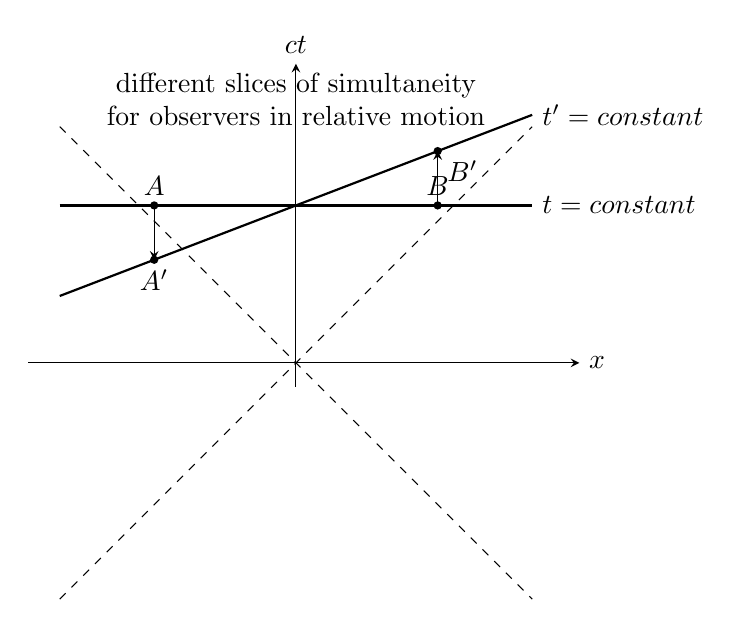
\begin{tikzpicture}[x=1cm,y=1cm,>=stealth]
    \draw[->] (-3.4,0) -- (3.6,0) node[right] {\(x\)};
    \draw[->] (0,-0.3) -- (0,3.8) node[above] {\(ct\)};

    \draw[dashed] (-3,-3) -- (3,3);
    \draw[dashed] (-3,3) -- (3,-3);

    % laboratory simultaneity
    \draw[thick] (-3,2.0) -- (3,2.0) node[right] {\(t=\text{constant}\)};
    \fill (-1.8,2.0) circle (1.5pt) node[above] {\(A\)};
    \fill (1.8,2.0) circle (1.5pt) node[above] {\(B\)};

    % moving-frame simultaneity, ct' constant: ct - beta x = const
    \draw[thick] (-3,0.85) -- (3,3.15) node[right] {\(t'=\text{constant}\)};
    \fill (-1.8,1.31) circle (1.5pt) node[below] {\(A'\)};
    \fill (1.8,2.69) circle (1.5pt) node[below right] {\(B'\)};

    \draw[->] (-1.8,2.0) -- (-1.8,1.31);
    \draw[->] (1.8,2.0) -- (1.8,2.69);
    \node[align=center] at (0,3.35) {different slices of simultaneity\\for observers in relative motion};
\end{tikzpicture}

\caption{Lines of simultaneity differ between inertial frames. A horizontal line
is simultaneous in the laboratory frame, while a tilted line is simultaneous in
a moving frame.}
\end{figure}

This effect is not an optical illusion caused by signal travel time. It remains
after correcting for the time light takes to reach the observer. It is a
structural statement about how inertial frames assign time coordinates to
distant events.

A common thought experiment uses a train and a platform. Two lightning strikes
hit the front and rear of a moving train. A platform observer at the midpoint
may judge the strikes simultaneous. A train observer at the train midpoint does
not: because the train observer moves toward one flash and away from the other,
and because light speed is the same in the train frame, the events cannot both
have occurred at equal train-frame times. The disagreement is not about what is
seen; it is about the time coordinates assigned to the events.

\clearpage

\section{Time Dilation}

Time dilation concerns two events that occur at the same place in the moving
clock's own rest frame. Let a clock be at rest in \(S'\). Two ticks have
\(\Delta x'=0\). The inverse Lorentz transformation gives
\[
\Delta t=\gamma\left(\Delta t'+\frac{v\Delta x'}{c^2}\right).
\]
Since \(\Delta x'=0\),
\[
\Delta t=\gamma\Delta t'.
\]
The time between ticks measured in the clock's own rest frame is the proper time
\(\Delta\tau=\Delta t'\). Thus
\[
\boxed{\Delta t=\gamma\Delta\tau.}
\]
A moving clock is measured to run slow: more coordinate time \(\Delta t\) passes
in the laboratory frame than proper time \(\Delta\tau\) passes on the moving
clock.

\begin{figure}[h]
\centering
\begin{tikzpicture}[x=1cm,y=1cm,>=Stealth]
  \draw[->] (-0.5,0) -- (5.4,0) node[right] {$x$};
  \draw[->] (0,-0.2) -- (0,4.6) node[above] {$ct$};

  \draw[thick] (0.9,0.2) -- (0.9,4.0);
  \fill (0.9,1.0) circle (1.4pt) node[left] {tick 1};
  \fill (0.9,3.2) circle (1.4pt) node[left] {tick 2};

  \draw[thick] (2.2,0.4) -- (4.1,4.2);
  \fill (2.55,1.1) circle (1.4pt) node[right] {tick 1};
  \fill (3.55,3.1) circle (1.4pt) node[right] {tick 2};

  \node[align=left,anchor=west] at (1.3,4.15)
    {Proper time is measured\\along one clock's worldline:\\$(c\Delta\tau)^2=(c\Delta t)^2-(\Delta x)^2$};
\end{tikzpicture}

\caption{Time dilation represented by two ticks on a moving clock's worldline.
The proper time is measured along the clock's own worldline.}
\end{figure}

The phrase ``moving clocks run slow'' must be used carefully. Each inertial
observer says that clocks moving relative to that observer run slow. This is not
a contradiction because the comparison of distant clocks depends on the frame's
notion of simultaneity. When acceleration and reunion are involved, as in the
twin paradox, the worldlines are not symmetric and the accumulated proper times
can differ.

\clearpage

\section{Length Contraction}

Length contraction concerns a rod at rest in \(S'\) with proper length \(L_0\).
Its endpoints have fixed coordinates \(x'_1\) and \(x'_2\), with
\[
L_0=x'_2-x'_1.
\]
To measure the rod's length in frame \(S\), one must record the positions of
both endpoints at the same time in \(S\). Therefore \(\Delta t=0\) for the two
measurement events.

Use the spatial Lorentz transformation
\[
\Delta x'=\gamma(\Delta x-v\Delta t).
\]
For a length measurement in \(S\), \(\Delta t=0\), so
\[
\Delta x'=\gamma\Delta x.
\]
Since \(\Delta x'=L_0\) and \(\Delta x=L\), we obtain
\[
\boxed{L=\frac{L_0}{\gamma}.}
\]
A moving rod is shorter along the direction of motion than its proper length.
Transverse lengths are unchanged by a boost along the \(x\)-axis.

\begin{figure}[h]
\centering
\begin{tikzpicture}[x=1cm,y=1cm,>=Stealth]
  \draw[->] (-0.3,0) -- (5.8,0) node[right] {$x$};
  \draw[->] (0,-0.2) -- (0,4.5) node[above] {$ct$};

  \draw[thick] (0.8,0.2) -- (2.2,4.2) node[above] {rear end};
  \draw[thick] (3.1,0.2) -- (4.5,4.2) node[above] {front end};

  \draw[very thick] (1.43,2.0) -- (3.73,2.0);
  \fill (1.43,2.0) circle (1.4pt);
  \fill (3.73,2.0) circle (1.4pt);
  \node[above] at (2.58,2.05) {$L=L_0/\gamma$};

  \draw[dashed] (1.02,0.82) -- (3.32,2.12);
  \node[below right] at (2.55,1.55) {$t'=\mathrm{const}$};
\end{tikzpicture}

\caption{Length contraction in a spacetime diagram. A length measurement compares
endpoint events that are simultaneous in the measuring frame.}
\end{figure}

The important conceptual point is that a length is not a property of a single
event. It is a relation between two endpoint events chosen according to a
simultaneity convention. Different inertial frames select different pairs of
endpoint events when they measure the length of a moving object.

\clearpage

\section{Proper Time and Worldlines}

For a particle moving with speed \(u(t)\) in a given inertial frame, its proper
time increment is
\[
d\tau=dt\sqrt{1-\frac{u^2}{c^2}}=\frac{dt}{\gamma_u},
\]
where
\[
\gamma_u=\frac{1}{\sqrt{1-u^2/c^2}}.
\]
Therefore the accumulated proper time along a worldline is
\[
\tau=\int d\tau=\int \sqrt{1-\frac{u(t)^2}{c^2}}\,dt.
\]
This formula is the mathematical core of the twin paradox. The elapsed time on a
physical clock is the proper time along its worldline. Different worldlines
connecting the same two events can have different proper times.

For inertial motion at constant speed \(u\), the expression reduces to
\[
\Delta\tau=\Delta t\sqrt{1-\frac{u^2}{c^2}}=\frac{\Delta t}{\gamma_u}.
\]
Thus the moving clock records less proper time than the coordinate time measured
in the chosen inertial frame.

In spacetime geometry, an inertial worldline is straight. An accelerated
worldline is curved. The difference in elapsed proper time is therefore not
caused by a mysterious biological or mechanical effect on clocks. It is a
geometric consequence of the spacetime interval.

\clearpage

\section{Four-Vectors}

A spacetime event is represented by the position four-vector
\[
x^\mu=(ct,x,y,z).
\]
With the chosen metric signature, the squared interval is
\[
x^\mu x_\mu=(ct)^2-x^2-y^2-z^2.
\]
The proper time allows us to define the four-velocity
\[
U^\mu=\frac{dx^\mu}{d\tau}.
\]
If the ordinary three-velocity is \(\mathbf{u}=d\mathbf{x}/dt\), then
\[
U^\mu=\gamma_u(c,u_x,u_y,u_z).
\]
Its invariant norm is
\[
U^\mu U_\mu=c^2.
\]
The four-momentum of a particle of rest mass \(m\) is
\[
p^\mu=mU^\mu=(\gamma mc,\gamma m\mathbf{u}).
\]
The energy and three-momentum are therefore
\[
E=\gamma mc^2,
\qquad
\mathbf{p}=\gamma m\mathbf{u}.
\]
Writing the four-momentum as
\[
p^\mu=\left(\frac{E}{c},\mathbf{p}\right),
\]
its invariant norm gives
\[
p^\mu p_\mu=\frac{E^2}{c^2}-p^2=m^2c^2.
\]
Multiplying by \(c^2\), we obtain the energy-momentum relation
\[
\boxed{E^2=p^2c^2+m^2c^4.}
\]
For a particle at rest, \(p=0\), and this reduces to
\[
\boxed{E_0=mc^2.}
\]
For a massless particle, \(m=0\), so
\[
E=pc.
\]

\clearpage

\section{Muon Lifetime as an Experimental Test}

Cosmic rays striking the upper atmosphere produce muons. A muon at rest has a
mean lifetime of approximately
\[
\tau_0\approx 2.2\,\mu\mathrm{s}.
\]
Classically, even if it moved almost at the speed of light, it would travel a
rough distance
\[
c\tau_0\approx (3.0\times 10^8\,\mathrm{m/s})(2.2\times 10^{-6}\,\mathrm{s})
\approx 660\,\mathrm{m}.
\]
Many muons are created several kilometres above Earth's surface, yet a
significant number are detected near the ground. Special relativity explains
this without contradiction.

In the Earth frame, the muon is moving rapidly, so its lifetime is dilated:
\[
\Delta t=\gamma\tau_0.
\]
If \(\gamma=10\), for example, then
\[
\Delta t\approx 22\,\mu\mathrm{s},
\]
and the possible travel distance is approximately
\[
L\approx c\Delta t\approx 6.6\,\mathrm{km}.
\]
This is now compatible with atmospheric distances.

In the muon's rest frame, the muon lifetime is not dilated; it is simply
\(\tau_0\). Instead, the atmosphere moves toward the muon and is length
contracted:
\[
L=\frac{L_0}{\gamma}.
\]
Thus a several-kilometre atmospheric distance in the Earth frame can become a
few hundred metres in the muon frame. Both descriptions agree about the physical
fact: the muon can reach the detector.

\begin{figure}[h]
\centering
\begin{tikzpicture}[x=1cm,y=1cm,>=Stealth]
  \draw[->] (-0.2,0) -- (6.2,0) node[right] {distance};
  \draw[->] (0,-0.2) -- (0,4.8) node[above] {time};

  \draw[thick] (0.7,4.1) -- (5.4,0.7);
  \fill (0.7,4.1) circle (1.4pt) node[above right] {created};
  \fill (5.4,0.7) circle (1.4pt) node[below right] {detected};

  \draw[dashed] (0.7,0.7) -- (5.4,0.7);
  \draw[dashed] (0.7,0.7) -- (0.7,4.1);

  \node[align=left,anchor=west] at (1.0,2.7)
    {Earth frame: lifetime dilates.\\Muon frame: atmosphere contracts.};
\end{tikzpicture}

\caption{Muon survival can be described either by time dilation in the Earth
frame or by length contraction in the muon frame. The observed event is the same.}
\end{figure}

\clearpage

\section{Velocity Addition}

Suppose an object moves with velocity \(u'=dx'/dt'\) in frame \(S'\), and frame
\(S'\) moves with velocity \(v\) relative to \(S\). From the inverse Lorentz
transformation,
\[
dx=\gamma(dx'+vdt'),
\]
\[
dt=\gamma\left(dt'+\frac{v}{c^2}dx'\right).
\]
Dividing gives
\[
u=\frac{dx}{dt}
=\frac{dx'+vdt'}{dt'+(v/c^2)dx'}.
\]
Divide numerator and denominator by \(dt'\):
\[
\boxed{u=\frac{u'+v}{1+u'v/c^2}.}
\]
If \(u'=c\), then
\[
u=\frac{c+v}{1+v/c}=c.
\]
Thus light still moves at speed \(c\). If \(|u'|<c\) and \(|v|<c\), the result
also satisfies \(|u|<c\). The formula therefore encodes the impossibility of
accelerating massive particles to or beyond the speed of light by combining
ordinary subluminal velocities.

For perpendicular components, the formulas are more subtle. If the boost is
along \(x\), then
\[
u_x=\frac{u'_x+v}{1+u'_xv/c^2},
\]
\[
u_y=\frac{u'_y}{\gamma(1+u'_xv/c^2)},
\qquad
u_z=\frac{u'_z}{\gamma(1+u'_xv/c^2)}.
\]
The transverse components are affected because time itself transforms.

\clearpage

\section{Low-Velocity Limit}

Every new physical theory must reproduce the older successful theory in the
appropriate domain. For special relativity, this domain is \(v\ll c\). If
\(\beta=v/c\ll 1\), then
\[
\gamma=\frac{1}{\sqrt{1-\beta^2}}
\approx 1+\frac{1}{2}\beta^2.
\]
The Lorentz transformation becomes
\[
x'=\gamma(x-vt)\approx x-vt,
\]
while
\[
t'=\gamma\left(t-\frac{vx}{c^2}\right)
\approx t-rac{vx}{c^2}.
\]
For ordinary velocities and laboratory distances, the correction \(vx/c^2\) is
usually extremely small, so \(t'\approx t\). Hence the Galilean transformation
is recovered as an approximation.

This limiting argument is essential pedagogically. Special relativity does not
say that Newtonian mechanics was useless. It says that Newtonian mechanics is a
low-speed approximation to a deeper spacetime structure.

\clearpage

\section{Common Misinterpretations}

First, length contraction is not ordinary mechanical compression. A moving rod
does not feel squeezed in its own rest frame. Its proper length is still
\(L_0\). The contracted length appears when another inertial frame measures the
positions of the endpoints simultaneously in that other frame.

Second, time dilation is not due to poor clock construction. All ideal clocks
moving along the same worldline measure the same proper time. Atomic clocks,
mechanical clocks, biological aging, and unstable particle lifetimes are all
controlled by the same spacetime geometry.

Third, simultaneity is frame-dependent for spatially separated events. This does
not mean that causality is arbitrary. Events that can be causally connected have
timelike or lightlike separation, and their time order is preserved in all
inertial frames.

Fourth, the speed of light is not merely the speed of one particular object. It
is the invariant speed defining the causal structure of Minkowski spacetime.
Massless particles move at this speed in vacuum; massive particles have timelike
worldlines and move at speeds less than \(c\).

\clearpage

\section{Summary of Core Formulas}

The basic definitions are
\[
\beta=\frac{v}{c},
\qquad
\gamma=\frac{1}{\sqrt{1-\beta^2}}.
\]
The Lorentz transformation in standard configuration is
\[
x'=\gamma(x-vt),
\qquad
 t'=\gamma\left(t-\frac{vx}{c^2}\right),
\]
with inverse
\[
x=\gamma(x'+vt'),
\qquad
 t=\gamma\left(t'+\frac{vx'}{c^2}\right).
\]
The invariant interval is
\[
\Delta s^2=c^2\Delta t^2-\Delta x^2-\Delta y^2-\Delta z^2.
\]
For timelike intervals,
\[
\Delta s^2=c^2\Delta\tau^2.
\]
Time dilation is
\[
\Delta t=\gamma\Delta\tau.
\]
Length contraction is
\[
L=\frac{L_0}{\gamma}.
\]
Relativity of simultaneity follows from
\[
\Delta t'=\gamma\left(\Delta t-\frac{v\Delta x}{c^2}\right).
\]
The velocity addition formula is
\[
u=\frac{u'+v}{1+u'v/c^2}.
\]
The energy-momentum relation is
\[
E^2=p^2c^2+m^2c^4.
\]
These formulas are not independent tricks. They are consequences of the single
geometric principle that inertial transformations preserve the Minkowski
spacetime interval.

\begin{summarybox}
Special relativity replaces separate absolute space and absolute time with
Minkowski spacetime. Lorentz transformations preserve the interval
\(c^2dt^2-dx^2-dy^2-dz^2\). Time dilation, length contraction, relativity of
simultaneity, velocity addition, and relativistic energy-momentum all follow
from this invariant structure.
\end{summarybox}
